\documentclass[12pt]{article}
\usepackage[portuguese]{babel}
\usepackage[utf8]{inputenc}
%\usepackage{citesort} % sorts citation numbers appropriately
\usepackage[]{graphicx} % use this when importing ps- and eps-files
\usepackage{url}
\usepackage{listings}
% \usepackage[pdftex]{graphicx} % use this when importing PDF files

% horizontal margins: 1.0 + 6.5 + 1.0 = 8.5
\setlength{\oddsidemargin}{0.0in}
\setlength{\textwidth}{6.5in}
% vertical margins: 1.0 + 9.0 + 1.0 = 11.0
\setlength{\topmargin}{0.0in}
\setlength{\headheight}{12pt}
\setlength{\headsep}{13pt}
\setlength{\textheight}{625pt}
\setlength{\footskip}{24pt}

\pagestyle{myheadings}

\title{\bfseries Simulação de ecossistemas em memória partilhada usando \textit{pipelines}}
\author{Flávio Manuel Fernandes Cruz}
\date{12 de Dezembro de 2009}

\begin{document}

\maketitle

\subparagraph{Resumo.} A paralelização da simulação de um ecossistema pode ser resolvida usando diversas estratégias.
Neste relatório
será descrita uma solução em memória partilhada que usa o paradigma de \textit{pipelining} para simular um sistema
de raposas e coelhos. Os algoritmos e estruturas de dados utilizados serão analisados e os resultados
obtidos em termos temporais serão comparados com uma versão sequencial.

\section{Introdução}

Neste relatório será descrita uma solução para o problema de simular, de forma paralela,
sucessivas gerações de um eco-sistema composto por raposas e coelhos.

O eco-sistema é representado por uma matriz onde
cada posição pode ser ocupada por um coelho, uma raposa ou um rocha.
A matriz é inicializada por uma população inicial de coelhos e raposa.
Diversas rochas serão colocadas para funcionar como obstáculos.

A evolução do eco-sistema é feita geração a geração de acordo com um conjunto de regras bem definido.
A simulação termina quando um determinado número de gerações é atingido.

Foi implementada uma versão sequencial para o problema e outra versão paralela em memória partilhada
que funciona usando o paradigma de \textit{pipelining}.

O resto deste relatório será composto pela descrição das regras do sistema e da descrição
ds algoritmos e estruturas de dados comuns e específicos para cada versão.
Os aspectos relativos à divisão de trabalho, sincronização e balanceamento de carga
serão do foco principal da análise da versão paralela.
De seguida, serão mostrados resultados em termos de tempo
e \textit{speedup} da versão paralela em relação à versão sequencial. Finalmente,
o relatório terminará com uma pequena conclusão e análise dos resultados obtidos.

\section{Regras}

O eco-sistema é representado por uma matriz de \textbf{LIN} linhas e \textbf{COL} colunas.
Cada posição é ocupada por um coelho, uma raposa ou uma rocha.
A simulação é feita gerando sucessivas gerações do sistema até se atingir o número
desejado de gerações.

Por cada geração os coelhos movem-se segundo as seguintes regras \cite{enunciado}:

\begin{itemize}
  \item Os coelhos tentam mover-se para um dos espaços adjacentes livres. Se existirem vários espaços adjacentes livres, escolhem um deles segundo um determinado critério. Se não existir nenhum espaço adjacente livre, mantêm-se no mesmo lugar.
  \item Os coelhos podem mover-se na horizontal e na vertical mas não na diagonal.
  \item Os coelhos podem procriar sempre que passarem \textbf{GER\_PROC\_COELHOS} gerações desde que nasceram ou desde que procriaram pela última vez. Depois de atingir a idade de procriar, quando posteriormente um coelho se move, este deixa na sua posição anterior um novo coelho de idade 0. A sua idade para procriar volta a 0.
\end{itemize}

Já as raposas seguem as seguintes regras \cite{enunciado}:

\begin{itemize}
  \item A cada geração, as raposas tentam comer coelhos movendo-se para espaços adjacentes que estejam ocupados por coelhos. Se existirem vários espaços adjacentes ocupados por coelhos, escolhem um deles segundo um determinado critério. Se não existir nenhum espaço adjacente ocupado por coelhos, as raposas tentam mover-se para um dos espaços adjacentes livres, utilizando o mesmo critério de escolha no caso de existirem vários espaços livres. Se não existir nenhum espaço adjacente ocupado por coelhos ou livre, mantêm-se no mesmo lugar.
  \item As raposas podem mover-se na horizontal e na vertical mas não na diagonal.
  \item As raposas podem procriar sempre que passam \textbf{GER\_PROC\_RAPOSAS} gerações desde que nasceram ou desde que procriaram pela última vez. Depois de atingirem a idade de procriar, quando posteriormente uma raposa se move, esta deixa na sua posição anterior uma nova raposa de idade 0. A idade da raposa que se move volta a 0.
  \item As raposas morrem se não se alimentarem durante \textbf{GER\_ALIM\_RAPOSAS} gerações desde que nasceram ou desde que comeram um coelho pela última vez. As raposas não comem outras raposas, apenas coelhos.
\end{itemize}

Uma rocha nunca se move e funciona como obstáculo para as raposas e coelhos.

Ao seleccionar posições adjacentes é preciso ter em conta as seguintes regras \cite{enunciado}:

\begin{itemize}
  \item Numerar a partir de 0 e seguindo a ordem dos ponteiros do relógio, os possíveis \textbf{P} espaços adjacentes para onde é possível um coelho ou uma raposa se movimentar: espaço adjacente acima, espaço adjacente à direita, espaço adjacente abaixo e espaço adjacente à esquerda.
  \item Seja \textbf{G} a geração actual e sejam \textbf{(X,Y)} as coordenadas do espaço em que o coelho ou a raposa se encontra, então o novo espaço a seleccionar é determinado por \textbf{(G+X+Y) mod P}. Considere que a geração inicial (antes de qualquer movimentação) é a 0 e que a origem da matriz é \textbf{(0,0)}.
\end{itemize}

Quando um espaço é ocupado por mais de um animal ao mesmo tempo é necessário resolver o conflito de acordo com
as regras seguintes \cite{enunciado}:
\begin{itemize}
  \item Quando 2 ou mais coelhos se movimentam para o mesmo espaço livre, o coelho com o maior valor de idade (valor mais perto de \textbf{GER\_PROC\_COELHOS}) fica, os outros desaparecem.
  \item Quando 2 ou mais raposas se movimentam para comer o mesmo coelho, a raposa com o maior valor de idade (valor mais perto de \textbf{GER\_PROC\_RAPOSAS}) fica, as outras desaparecem.
  \item Quando 2 ou mais raposas se movimentam para o mesmo espaço livre, a raposa com mais fome (valor mais próximo de \textbf{GER\_ALIM\_RAPOSAS}) fica, as outras desaparecem. No caso de existirem 2 ou mais raposas com o mesmo valor de fome, fica aquela com o maior valor de idade (valor mais perto de \textbf{GER\_PROC\_RAPOSAS}).
\end{itemize}

\section{Arquitectura do sistema} \label{sec:arq}

O sistema foi dividido em diferentes blocos de funções e estruturas de dados que são
utilizados por 3 programas diferentes:

\begin{itemize}
  \item \textbf{seq}: versão \textit{puramente} sequencial do programa.
  \item \textbf{simulator}: versão paralela. Aceita um número de \textit{threads} como argumento.
  \item \textbf{generator}: gerador de mapas aleatórios.
\end{itemize}

\subsection{Módulos}

Foi criado o módulo \textbf{object} que encapsula a criação de estruturas do
tipo \textit{Fox} e \textit{Rabbit}, estas têm como base uma estrutura de nome \textit{Object}.
Cada uma destas estruturas contém assim o tipo de objecto e estado adicional necessário para correr a simulação:

\begin{itemize}
  \item \textit{Rabbit}
  \begin{itemize}
    \item last\_procreation: tempo desde a última procriação.
  \end{itemize}
  \item \textit{Fox}
  \begin{itemize}
    \item last\_procreation: tempo desde a última procriação.
    \item last\_food: tempo desde a última vez que a raposa comeu um coelho.
  \end{itemize}
\end{itemize}

Para guardar o estado de um sistema/mapa foi criado o módulo \textbf{map}. Este
contém a descrição da estrutura de dados para um mapa e respectivas funções que lêm,
escrevem e geram mapas. Cada objecto do tipo mapa contém, entre outras informações,
os seguintes atributos:

\begin{itemize}
  \item ger\_proc\_coelhos: número de gerações necessárias para um coelho se reproduzir.
  \item ger\_proc\_raposas: número de gerações necessárias para uma raposa se reproduzir.
  \item ger\_alim\_raposas: quando uma raposa passa este número de gerações sem se alimentar, morre.
  \item n\_ger: número de gerações a simular.
  \item lin: número de linhas.
  \item col: número de colunas.
  \item matriz de posições: matriz de objectos do tipo \textit{Position}, com informação para cada posição da matriz.
\end{itemize}

Cada posição do mapa é implementada pelo módulo \textbf{position}. O objecto posição contém
um booleano que indica se a posição é uma rocha, e, em caso contrário, um apontador para um objecto do tipo \textit{Object}.

Para simular uma geração de forma sequencial é utilizado o módulo \textbf{thread}. Cada geração
funciona por duas iterações completas pela matriz do mapa:

\begin{itemize}
  \item Num primeiro passo (\textit{thread\_simulate\_position}) é verificado se existe algum objecto
  na posição actual e dependendo do tipo, coelho ou raposa, são executadas algumas regras da simulação:
    \begin{itemize}
      \item Coelhos: é incrementado o tempo de procriação (\textit{last\_procreation}) e feita a pesquisa por uma posição
        adjacente que não tenha objectos, para onde será movido.
        Caso seja necessário que o coelho se reproduza, o novo coelho é mantida na posição
        actual.
      \item Raposas: a lógica é idêntica para as raposas, embora seja necessário verificar se a raposa vai morrer de fome.
       A procura por um espaço adjacente para a movimentação é feita no sentido de encontrar um espaço com um coelho.
    \end{itemize}
    Neste primeiro passo nenhum animal é colocado numa posição definitiva, sendo usado uma área de dados
    especial para cada posição onde se faz o registo das movimentações para o passo 2 desta geração.
  \item No segundo passo (\textit{thread\_resolve\_conflicts}) é analisada a área de dados de movimentações de cada posição e são resolvidos os conflitos.
\end{itemize}

\subsection{Movimentação}

Durante a primeira fase são usadas as funções \textit{position\_move\_fox} e \textit{position\_move\_rabbit}
onde é usado o estado temporário da posição para onde o animal se irá mover. Este estado temporário
contém um vector onde são colocados animais que durante esta geração serão libertados da memória durante
o segundo passo. Também existem vários apontadores:

\begin{itemize}
  \item \textit{oldest\_fox}: apontador para a raposa mais antiga. Caso se movimentem diversas raposas para esta
    posição, este apontador irá sempre apontar para a raposa mais antiga.
  \item \textit{hungriest\_fox}: apontador para a raposa com mais fome que foi movida para esta posição neste turno.
  Caso se mova algum coelho durante a geração para esta posição, este apontador fica nulo, pois apenas a raposa mais
  velha ganha neste tipo de conflitos.
  \item \textit{best\_rabbit}: apontador para o coelho com mais idade. Quando é movida alguma raposa para
  esta posição este apontador deixa de ser usado e o coelho, caso exista, é colocado no vector de libertação de animais.
\end{itemize}

No final do primeiro passo existem três tipos de estado para estes apontadores:

\begin{itemize}
  \item Só o \textit{best\_rabbit} aponta: apenas coelhos se movimentaram para esta posição.
  \item Só o \textit{oldest\_fox} aponta: pelo menos um coelho também se tentou mover para esta posição e foi comido.
  \item Ambos \textit{oldest\_fox} e \textit{hungriest\_fox} não estão nulos: será escolhida a raposa com mais fome no segundo passo.
  \item Tudo a nulo: nenhum animal se movimentou para aqui.
\end{itemize}

O objecto principal deste sistema de apontadores é resolver os conflitos o mais cedo possível.

Quando finalmente o segundo passo do algoritmo é executado, o apontador para o objecto da posição é alterado
para respeitar o estado da área temporária e todos os objectos que devem ser libertados apartir desta posição são retirados da memória.

\section{Versão sequencial}

A versão sequencial do sistema faz uso dos módulos mencionados na secção \ref{sec:arq} (Arquitectura do sistema).

\begin{lstlisting}[language=c,frame=single,caption={Algoritmo da versão sequencial.},label=sequencial]
- De 0 ate a geracao limite:
  - Para todas as posicoes da matriz:
    thread_simulate_position(posicao) // simular movimentacao na posicao
  - Para todas as posicoes da matriz:
    thread_resolve_conflict(posicao) // resolver conflictos
\end{lstlisting}

As funções mencionadas na listagem \ref{sequencial} serão também utilizadas sem alterações na versão
paralela como veremos a seguir.

\section{Versão paralela}

A versão paralela da aplicação é feita em memória partilhada usando \textit{pthreads}.

A divisão do trabalho entre \textit{threads} é feita num sistema de fila de tarefas central, sendo
uma tarefa um bloco potencialmente variável de linhas da matriz, sendo a tarefa executar o primeiro
ou segundo passo do algoritmo mostrado anteriormente nesse bloco de linhas. A figura \ref{fig:tasks_matriz}
mostra uma possível divisão de uma matriz.

\begin{figure}[ht]
  \centering
    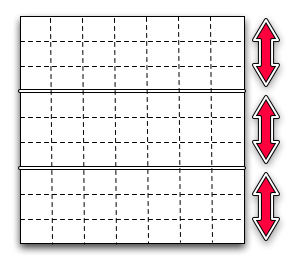
\includegraphics[scale=0.8]{diagrama_pipeline.png}
  \caption{Separação da matriz em blocos de linhas}
  \label{fig:tasks_matriz}
\end{figure}

À estrutura de dados \textit{Map} foram adicionados um \textit{mutex}, uma variável de condição
e as seguintes três variáveis booleanas:

\begin{itemize}
  \item \textit{proceed\_first\_pass}: indica se é possível avançar com novo trabalho
  para o primeiro passo do algoritmo.
  \item \textit{proceed\_second\_pass}: indica se é possível avançar com novo trabalho
  para o segundo passo do algoritmo.
  \item \textit{the\_end}: indica se o algoritmo terminou de computar, fazendo com que a \textit{thread} termine.
\end{itemize}

Inicialmente \textit{proceed\_first\_pass} encontra-se definido como verdadeiro para a primeira \textit{thread}
poder avançar. Cada mapa contém ainda um registo da geração em que cada linha se encontra para os dois passos
dos algoritmos, assim, quando é feita a verificação de novo trabalho, são verificadas as condições necessárias
para se poder avançar comparando os valores da geração nas linhas. É mantido também o registo
do número da linha fronteira para cada passo e a sua geração.

A selecção do número de linhas é feita usando um número de linhas previamente definido, caso
esse número exceda as linhas restantes da matriz, apenas são usadas as linhas que faltam.

\begin{lstlisting}[language=c,basicstyle=\footnotesize,frame=single,caption={Algoritmo paralelo.},label=algoritmo_paralelo]
- Repetir:
  - lock(map->mutex)
  - enquanto nao existirem tarefas ou o algoritmo tenha terminado:
    pthread_cond_wait(map->cond, map->mutex)
  - se o algoritmo terminou sair
  - se a tarefa for para o segundo passo do algoritmo:
    - calcular numero de linhas para esta tarefa
    - calcular a geracao para esta tarefa
    - se a geracao tiver atingido o limite pretendido e a linha for a inicial:
      - indicar que nao ha mais tarefas no segundo passo
    - se existirem mais tarefas para este passo:
      - verificar se e possivel sinalizar nova tarefa para o segundo passo do algoritmo
    - unlock(map->mutex)
    - fazer o segundo passo do algoritmo nas linhas obtidas:
      - thread_resolve_conflict(posicao)
      - actualizar geracao do segundo passo para a linha actual
    - se o algoritmo terminou sair
    - se este for o ultimo pedaco de linhas na ultima geracao:
      - the_end = TRUE
      - pthread_cond_broadcast(map->cond)
    - se existirem mais tarefas do primeiro passo:
      - lock(map->mutex)
      - tentar encontrar mais tarefas para o primeiro passo e sinalizar
      - unlock(map->mutex)
  - se a tarefa for para o primeiro passo do algoritmo:
    - calcular numero de linhas para esta tarefa
    - calcular a geracao para esta tarefa
    - se a geracao tiver atingido o limite pretendido e a linha for a inicial:
      - indicar que nao ha mais tarefas no primeiro passo
    - se existirem mais tarefas para este passo:
      - tentar verificar que e possivel avancar no primeiro passo
    - unlock(map->mutex)
    - executar o primeiro passo no bloco atribuido:
      - thread_simulate_position(posicao)
      - actualizar geracao do primeiro passo para a linha actual
    - se algoritmo terminou sair
    - se for possivel avancar no segundo passo:
      - lock(map->mutex)
      - tentar encontrar mais tarefas para o segudno passo e sinalizar
      - unlock(map->mutex)
\end{lstlisting}

Pelo algoritmo ilustrado na listagem \ref{algoritmo_paralelo} podemos verificar que o sistema
irá adoptar um comportamento baseado numa \textit{pipeline}, onde cada \textit{thread} não terá
nenhum conjunto de linhas atribuído por defeito, sendo possível que num mesmo mapa uma parte esteja
a simular a geração \textit{N} e noutra parte a geração \textit{N - 1}.
Este efeito pode ser visto graficamente na Figura \ref{fig:evolucao}, onde a cor laranja
são tarefas do primeiro passo, a azul do segundo passo.

\begin{figure}[ht]
  \centering
    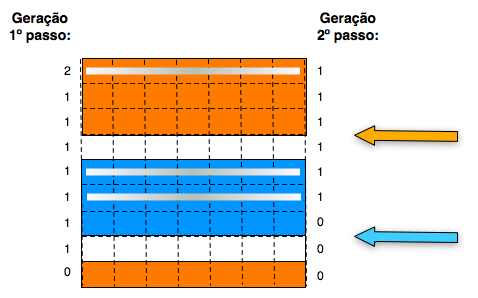
\includegraphics[scale=0.8]{diagrama_evolucao.png}
  \caption{Execução do algoritmo paralelo com três threads.}
  \label{fig:evolucao}
\end{figure}

Pela Figura \ref{fig:evolucao} podem-se também ver os apontadores das tarefas para ambos os passos (setas do lado direito)
e de cada lado o número da geração para a respectiva linha. Por exemplo, quando a 2ª tarefa (a azul) terminar,
esta irá verificar se é possível sinalizar nova tarefa do primeiro passo, o que se irá verificar,
pois as gerações de ambos os passos para o próximo bloco de tamanho 3 são iguais (geração 1), o que possibilita
a execução do primeiro passo para essa zona. 

Quando se pretende verificar que se pode avançar o apontador das tarefas do segundo passo, é necessário
que todas as linhas sejam da geração \textit{N} no primeiro passo e da geração \textit{N - 1} para o segundo
passo.

Estas verificações são feitas para o bloco que se pretende obter mas também para uma linha à frente, de forma
a que um bloco de linhas do primeiro passo nunca pode esteja colado a um bloco do segundo passo devido à
movimentação dos animais durante o primeiro passo, o que tornaria os resultados inconsistentes.

Foram necessárias outras alterações no código partilhado entre a versão sequencial e paralela, nomeadamente,
a adição de um \textit{mutex} para cada posição da matriz. Este é usado para proteger a movimentação
de um animal para essa posição e toda a gestão da área temporária de dados.

Em termos de divisão de trabalho e balanceamento de carga, a natureza do algoritmo implementado
assegura que na grande maioria dos casos nenhuma \textit{thread} irá ter trabalho a mais,
desde que a divisão em blocos do mapa seja adequado para o número de \textit{threads} e tamanho do eco-sistema.
Isto permite que todas as \textit{threads} estejam constantemente a computar e a processar
novas tarefas. Não esquecer que no esquema descrito, todas as \textit{threads} têm a mesma oportunidade
para trabalhar, resultando numa boa distribuição de carga.

\section{Resultados}

Durante a implementação da solução foi-se verificando que a definição do tamanho do bloco de linhas
para cada tarefa afectava de forma bastante significativa a performance do algoritmo paralelo.
Por exemplo, se o tamanho do bloco for demasiado pequeno, o sistema irá passar demasiado tempo
a computar se é possível avançar para as próximas tarefas, já um tamanho demasiado grande,
fará com que algumas \textit{threads} fiquem bloqueadas à espera de novas tarefas, dado que não será sempre
possível avançar devido às restrições entre o primeiro e segundo passo.

Decidiu-se experimentar diferentes funções para calcular o tamanho dos blocos em função do número de linhas
do mapa (\textbf{LIN}) e o número de \textit{threads} (\textbf{NTHREADS}).
Foram também criados 3 ficheiros de teste:

\begin{itemize}
  \item \textit{teste1}: mapa 100x100: 10000 gerações. 8968 animais.
  \item \textit{teste2}: mapa 500x100: 10000 gerações. 44973 animais.
  \item \textit{teste3}: mapa 1000x100: 10000 gerações. 90165 animais.
\end{itemize}

Para todos os eco-sistemas o número de gerações até que um coelho possa procriar é 1, o número
de gerações até que uma raposa possa procriar é 8 e o número de gerações até que uma raposa morra à fome é 3.

Os testes foram executados num computador com 4 processadores \textit{Intel(R) Xeon(TM) CPU 3.20GHz} e 6GB de
memória RAM.

\begin{table}[H]
    \begin{tabular}{ | l | c |}
      \hline
      \textbf{Teste} & \textbf{Time} \\ \hline
      1 (sequencial) & 0m20.776s \\ \hline
      1 (1 \textit{thread}) & 0m25.480s \\ \hline
      2 (sequencial) & 2m21.434s \\ \hline
      2 (1 \textit{thread}) & 2m44.494s \\ \hline
      3 (sequencial) & 5m6.016s \\ \hline
      3 (1 \textit{thread}) & 5m47.282s \\ \hline
  \end{tabular}
  \caption{Resultados para execuções sequenciais}
  \label{tbl:resultados_seq}
\end{table}

\begin{table}[H]
    \begin{tabular}{ | l | c | c | c | c |}
      \hline
      \textbf{Teste} & \textbf{\textit{Threads}} & \textbf{Time} & \textbf{Speedup / sequencial} & \textbf{Speedup / 1 thread}\\ \hline
      1 & 2 & 0m15.868s & 1.31 & 1.61 \\ \hline
      1 & 4 & 0m15.862s & 1.31 & 1.61 \\ \hline
      2 & 2 & 2m4.158s & 1.14 & 1.32 \\ \hline
      2 & 4 & 1m47.983s & 1.31 & 1.52 \\ \hline
      3 & 2 & 4m35.252s & 1.11 & 1.26 \\ \hline
      3 & 4 & 4m10.365s & 1.22 & 1.39 \\ \hline
  \end{tabular}
  \caption{Resultados para a função de divisão: LIN / (1.0 * NTHREADS)}
  \label{tbl:resultados1}
\end{table}

\begin{table}[H]
    \begin{tabular}{ | l | c | c | c | c |}
      \hline
      \textbf{Teste} & \textbf{\textit{Threads}} & \textbf{Time} & \textbf{Speedup / sequencial} & \textbf{Speedup / 1 thread}\\ \hline
      1 & 2 & 0m20.098s & 1.03 & 1.27 \\ \hline
      1 & 4 & 0m14.958s & 1.39 & 1.70 \\ \hline
      2 & 2 & 2m8.023s & 1.10 & 1.29 \\ \hline
      2 & 4 & 1m49.057s & 1.30 & 1.51 \\ \hline
      3 & 2 & 4m24.575s & 1.16 & 1.31 \\ \hline
      3 & 4 & 3m58.381s & 1.28 & 1.46 \\ \hline
  \end{tabular}
  \caption{Resultados para a função de divisão: LIN / (1.5 $*$ NTHREADS)}
  \label{tbl:resultados15}
\end{table}

\begin{table}[H]
    \begin{tabular}{ | l | c | c | c | c |}
      \hline
      \textbf{Teste} & \textbf{\textit{Threads}} & \textbf{Time} & \textbf{Speedup1} & \textbf{Speedup2}\\ \hline
      1 & 2 & 0m20.122s & 1.03 & 1.27 \\ \hline
      1 & 4 & 0m15.942s & 1.30 & 1.60 \\ \hline
      2 & 2 & 2m5.967s & 1.12 & 1.31 \\ \hline
      2 & 4 & 1m43.132s & 1.37 & 1.60 \\ \hline
      3 & 2 & 4m22.362s & 1.17 & 1.32 \\ \hline
      3 & 4 & 3m56.137s & 1.30 & 1.47 \\ \hline
  \end{tabular}
  \caption{Resultados para a função de divisão: LIN / (2.0 $*$ NTHREADS)}
  \label{tbl:resultados2}
\end{table}

\begin{table}[H]
    \begin{tabular}{ | l | c | c | c | c |}
      \hline
      \textbf{Teste} & \textbf{\textit{Threads}} & \textbf{Time} & \textbf{Speedup1} & \textbf{Speedup2}\\ \hline
      1 & 2 & 0m18.138s & 1.15 & 1.41 \\ \hline
      1 & 4 & 0m15.513s & 1.34 & 1.64 \\ \hline
      2 & 2 & 2m0.997s & 1.18 & 1.37 \\ \hline
      2 & 4 & 1m43.750s & 1.37 & 1.60 \\ \hline
      3 & 2 & 4m18.844s & 1.19 & 1.35 \\ \hline
      3 & 4 & 4m4.700s & 1.25 & 1.42 \\ \hline
  \end{tabular}
  \caption{Resultados para a função de divisão: LIN / (3.0 $*$ NTHREADS)}
  \label{tbl:resultados3}
\end{table}

\begin{table}[H]
    \begin{tabular}{ | l | c | c | c | c |}
      \hline
      \textbf{Teste} & \textbf{\textit{Threads}} & \textbf{Time} & \textbf{Speedup1} & \textbf{Speedup2}\\ \hline
      1 & 2 & 0m22.276s & 0.93 & 1.14 \\ \hline
      1 & 4 & 0m18.196s & 1.14 & 1.40 \\ \hline
      2 & 2 & 2m7.374s & 1.11 & 1.29\\ \hline
      2 & 4 & 1m33.914s & 1.51 & 1.75 \\ \hline
      3 & 2 & 4m21.648s & 1.17 & 1.33 \\ \hline
      3 & 4 & 4m0.389s & 1.28 & 1.45 \\ \hline
  \end{tabular}
  \caption{Resultados para a função de divisão: LIN / (5.0 $*$ NTHREADS)}
  \label{tbl:resultados5}
\end{table}

0m20.776s
0m25.480s
2m21.434s
2m44
5m6.016s
5m47.282s

\begin{table}[H]
    \begin{tabular}{ | l | c | c | c | c |}
      \hline
      \textbf{Teste} & \textbf{\textit{Threads}} & \textbf{Time} & \textbf{Speedup1} & \textbf{Speedup2}\\ \hline
      1 & 2 & 0m19.813s & 1.05 & 1.29 \\ \hline
      1 & 4 & 0m20.736s & 1.00 & 1.23 \\ \hline
      2 & 2 & 2m7.711s & 1.11 & 1.29 \\ \hline
      2 & 4 & 1m28.621s & 1.61 & 1.86 \\ \hline
      3 & 2 & 4m24.639s & 1.16 & 1.31 \\ \hline
      3 & 4 & 3m33.577s & 1.44 & 1.62 \\ \hline
  \end{tabular}
  \caption{Resultados para a função de divisão: LIN / (10.0 $*$ NTHREADS)}
  \label{tbl:resultados10}
\end{table}

\section{Conclusões}

\renewcommand{\bibname}{Referências}
\begin{thebibliography}{10}
  
	\bibitem{enunciado} Ricardo Rocha e Fernando Silva, Trabalho II: Simulação de um Ecossistema de Raposas e Coelhos, \url{http://www.dcc.fc.up.pt/~ricroc/aulas/0910/ppd/trabalhos/eco.html}
	
\end{thebibliography}

\bibliographystyle{plain}

\end{document}

